\section{Offline Reinforcement Learning}
Offline Reinforcement Learning is another paradigm of Reinforcement Learning. All previous 
methods we looked at are considered to be Online-RL methods. In Online-RL, the 
agent gathers data by directly interacting with the environment. It then uses this experience
immediately or via a replay buffer to update its policy, after which it has to interact with 
the environment again to collect more data.
\begin{figure}[H]
    \centering
    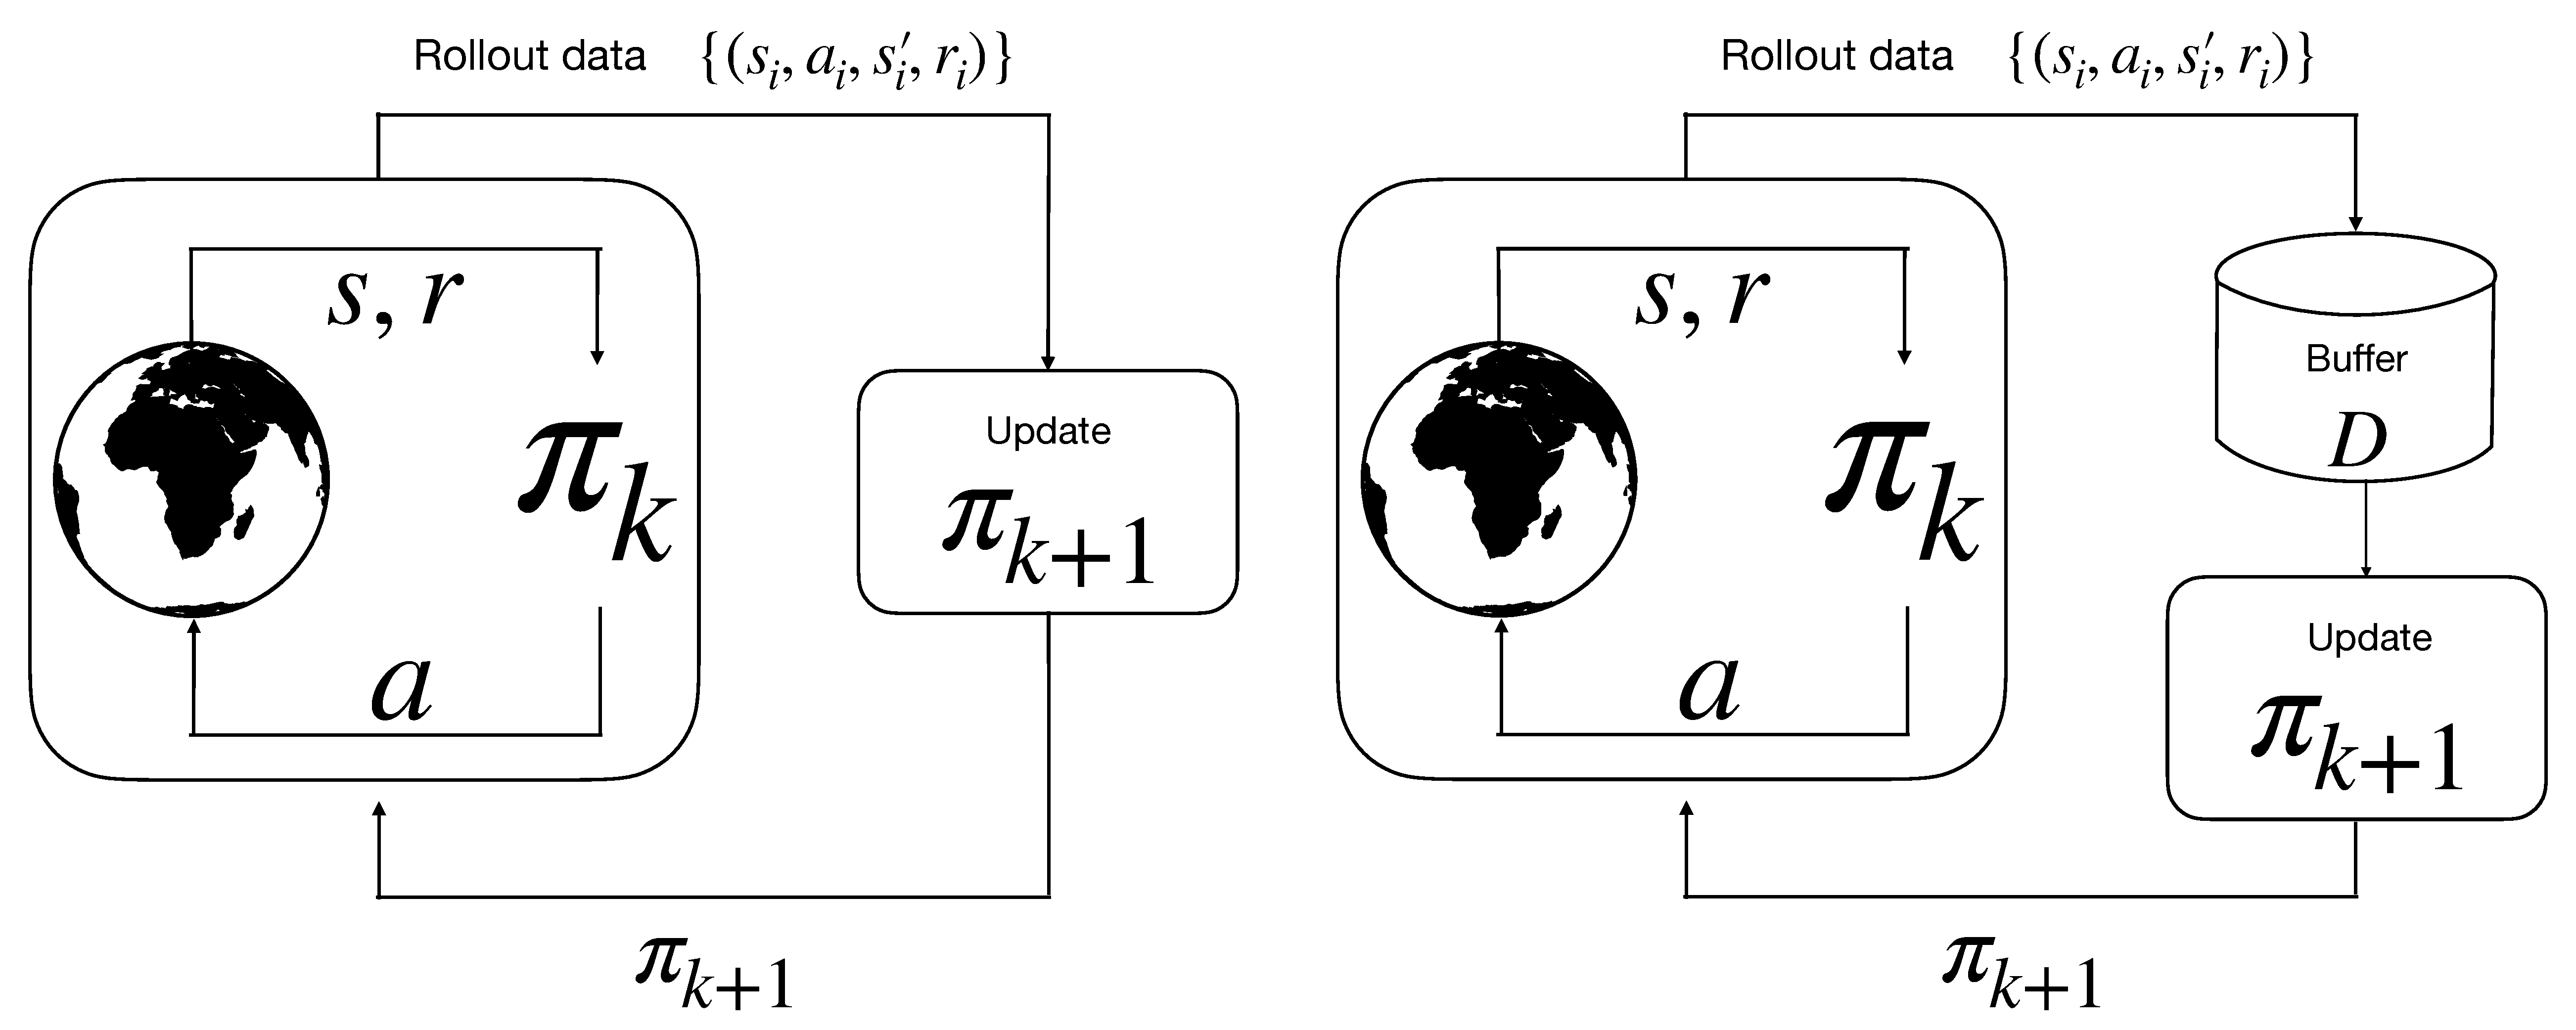
\includegraphics[width=0.8\linewidth]{images/off_vs_on_policy.pdf}
    \caption{Visualisation of online-RL as on-policy (left) and off-policy (right),inspired from 
    \cite{levine2020offlinereinforcementlearningtutorial}}
    \label{online_rl}
\end{figure}
Offline-RL is inspired by general deep learning. There we are just given a model and a 
large dataset to learn on. Throughout the training, the model does not interact in any way 
with anything outside the given data. But they are still able to generalise very well. In 
Offline-Rl, the agent only uses data collected from other agents and/or human 
demonstration to learn a policy, while not interacting with the environment once during 
training.
\vspace{-0.38cm}
\begin{figure} [H]
    \centering
    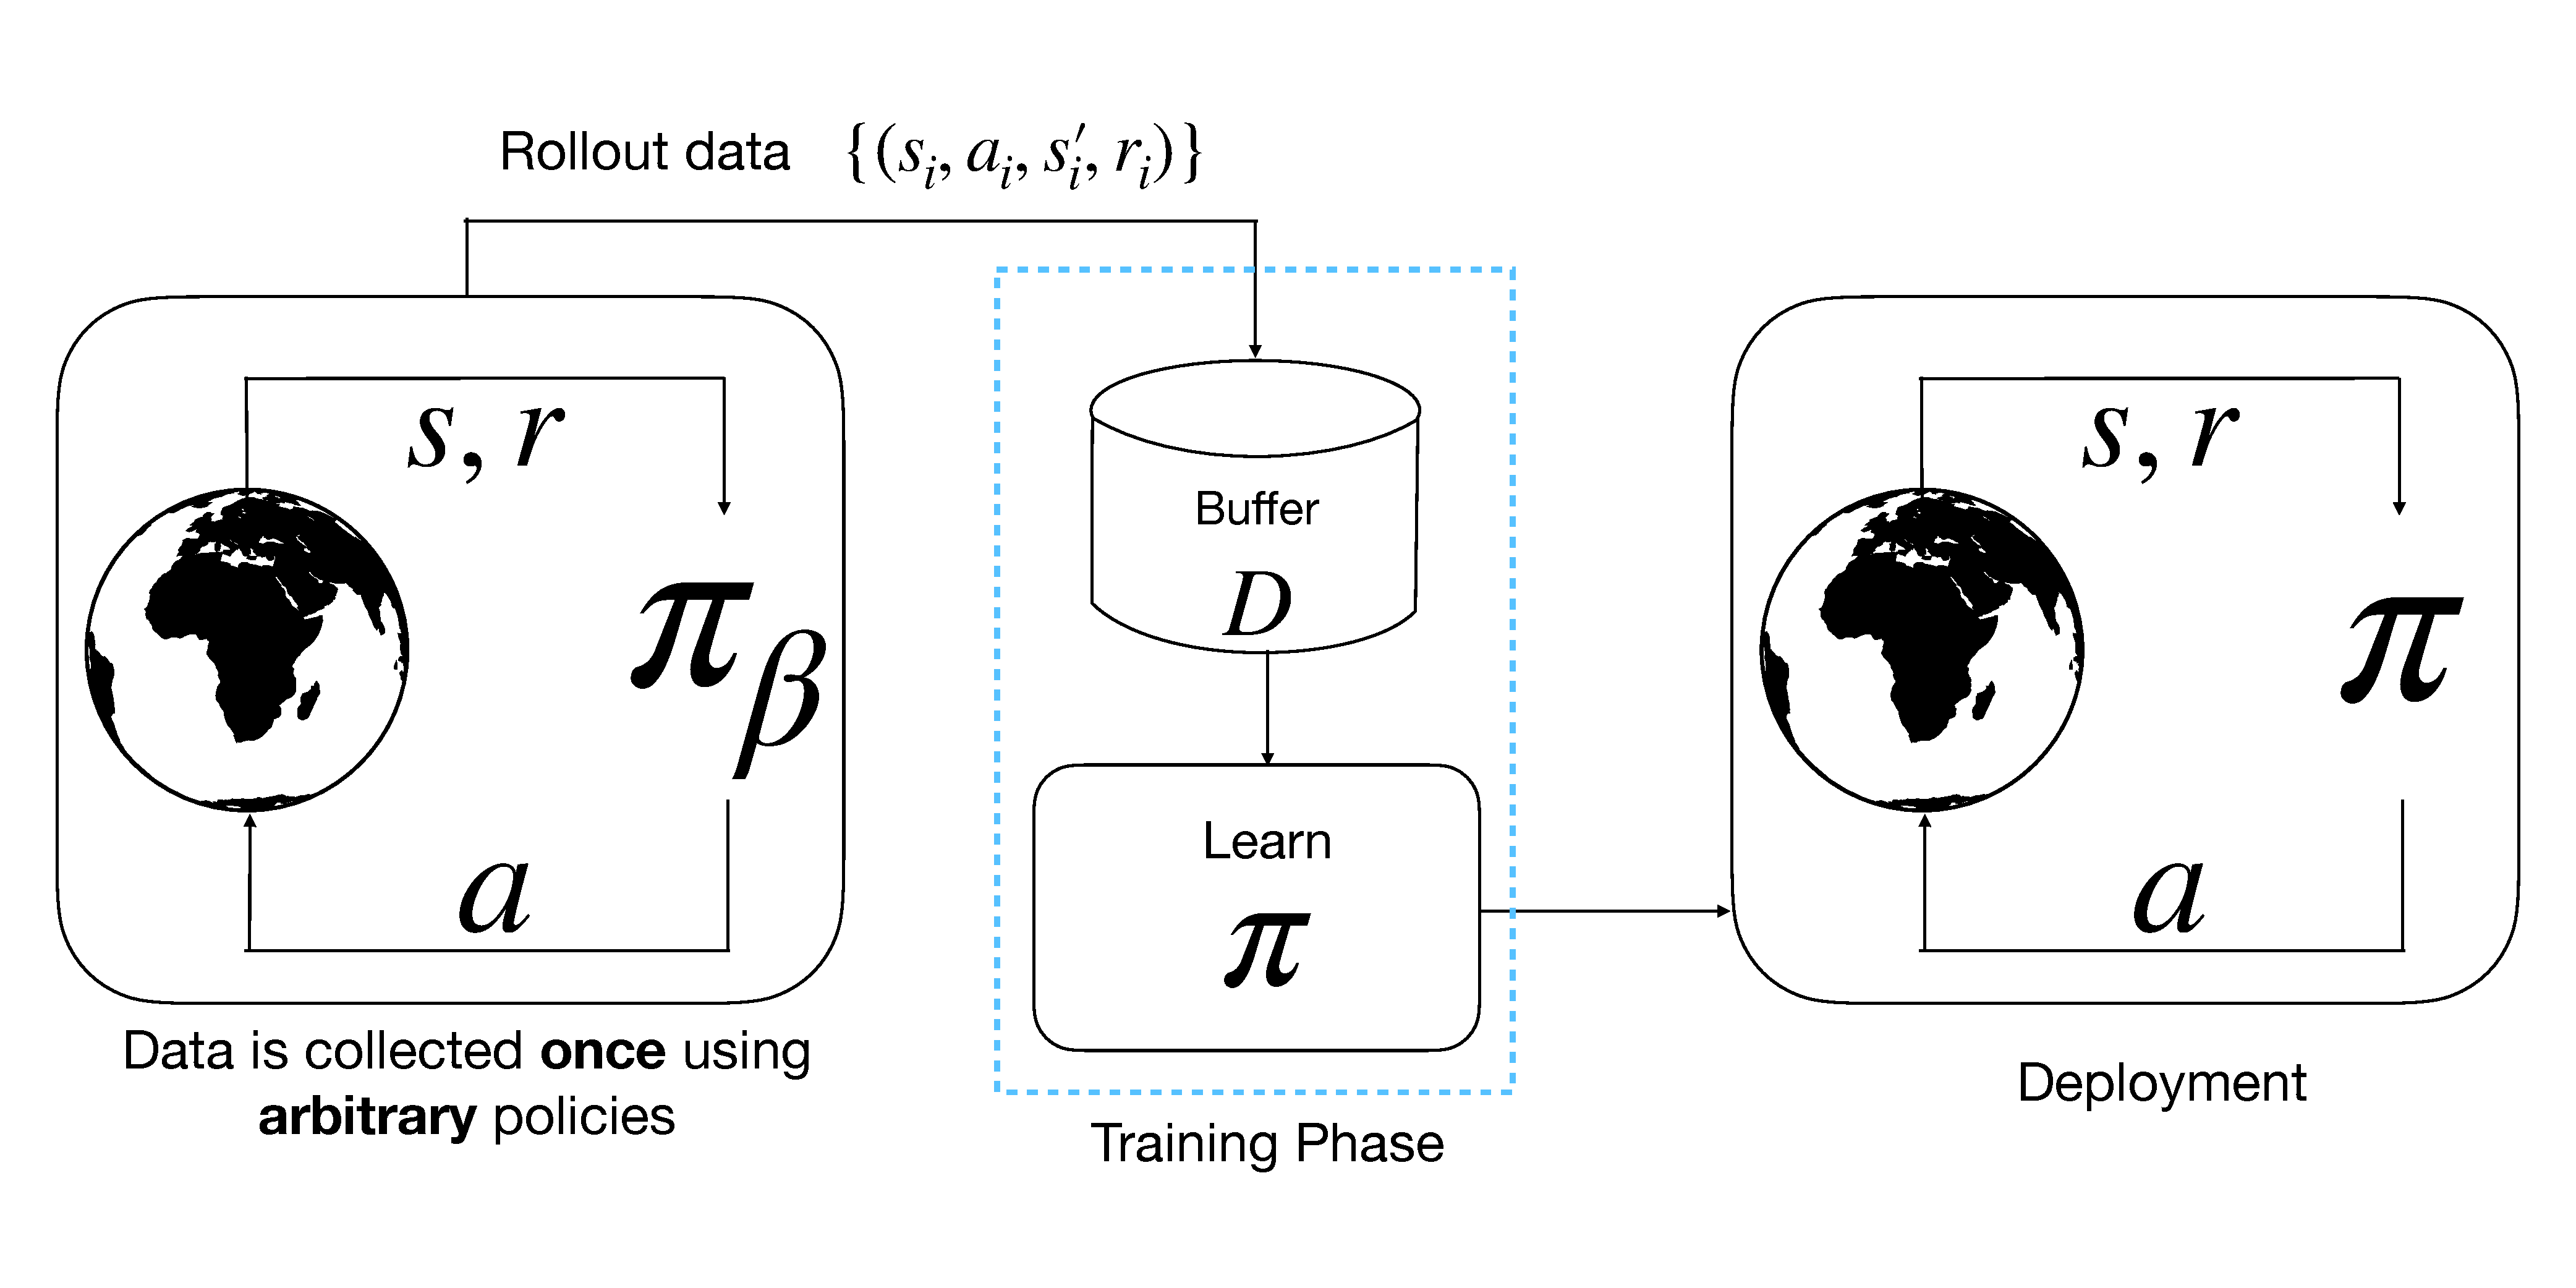
\includegraphics[width=0.8\linewidth]{images/offline_rl.pdf}
    \caption{Visualisation of Offline Reinforcement Learning, inspired from 
    \cite{levine2020offlinereinforcementlearningtutorial}}
    \label{offline_rl}
\end{figure}
In the following, we denote by $D$ the static dataset of transitions, defined as $D = \{(s_i, a_i, s_i', r_i)\}.$
The state-action tuples in this dataset are sampled such that the states $s$ are drawn from the stationary distribution 
$d^{\pi_\beta}(s)$ of a Markov chain (the distribution that remains unchanged over time under the dynamics induced by a 
policy). The actions $a$ are sampled from the behaviour policy $\pi_\beta(a \mid s)$, which is generally unknown.\newline
%The objective is then, as usual, to find the policy that maximises the expected sum of 
%discounted future rewards.
%$$\max\limits_\pi \underset{t=0}{\sum^T} \mathbb{E}_{s_t\sim d^\pi(s),a_t \sim \pi(a|s)}[\gamma^t r(s_t,a_t)]$$
The question that arises is whether we can hope to learn good policy without ever 
interacting with the environment. While we won’t formally prove it, the hope/claim is that
Offline RL can uncover the ''good stuff`` from a dataset that contains a mix of both good 
and bad behaviours. Importantly, the ''good stuff`` isn't limited to simply identifying the 
best trajectories in the dataset, but also includes the potential to learn policies that outperform
any single behaviour present in the data. This is based on the hope that Offline RL can generalize: 
that observing good behaviour in one context can inform good decisions in others. Ideally, the agent 
would be able to ''stitch together`` different pieces of good behaviour from across the dataset to construct 
an even better overall policy.
\begin{figure} [H]
    \centering
    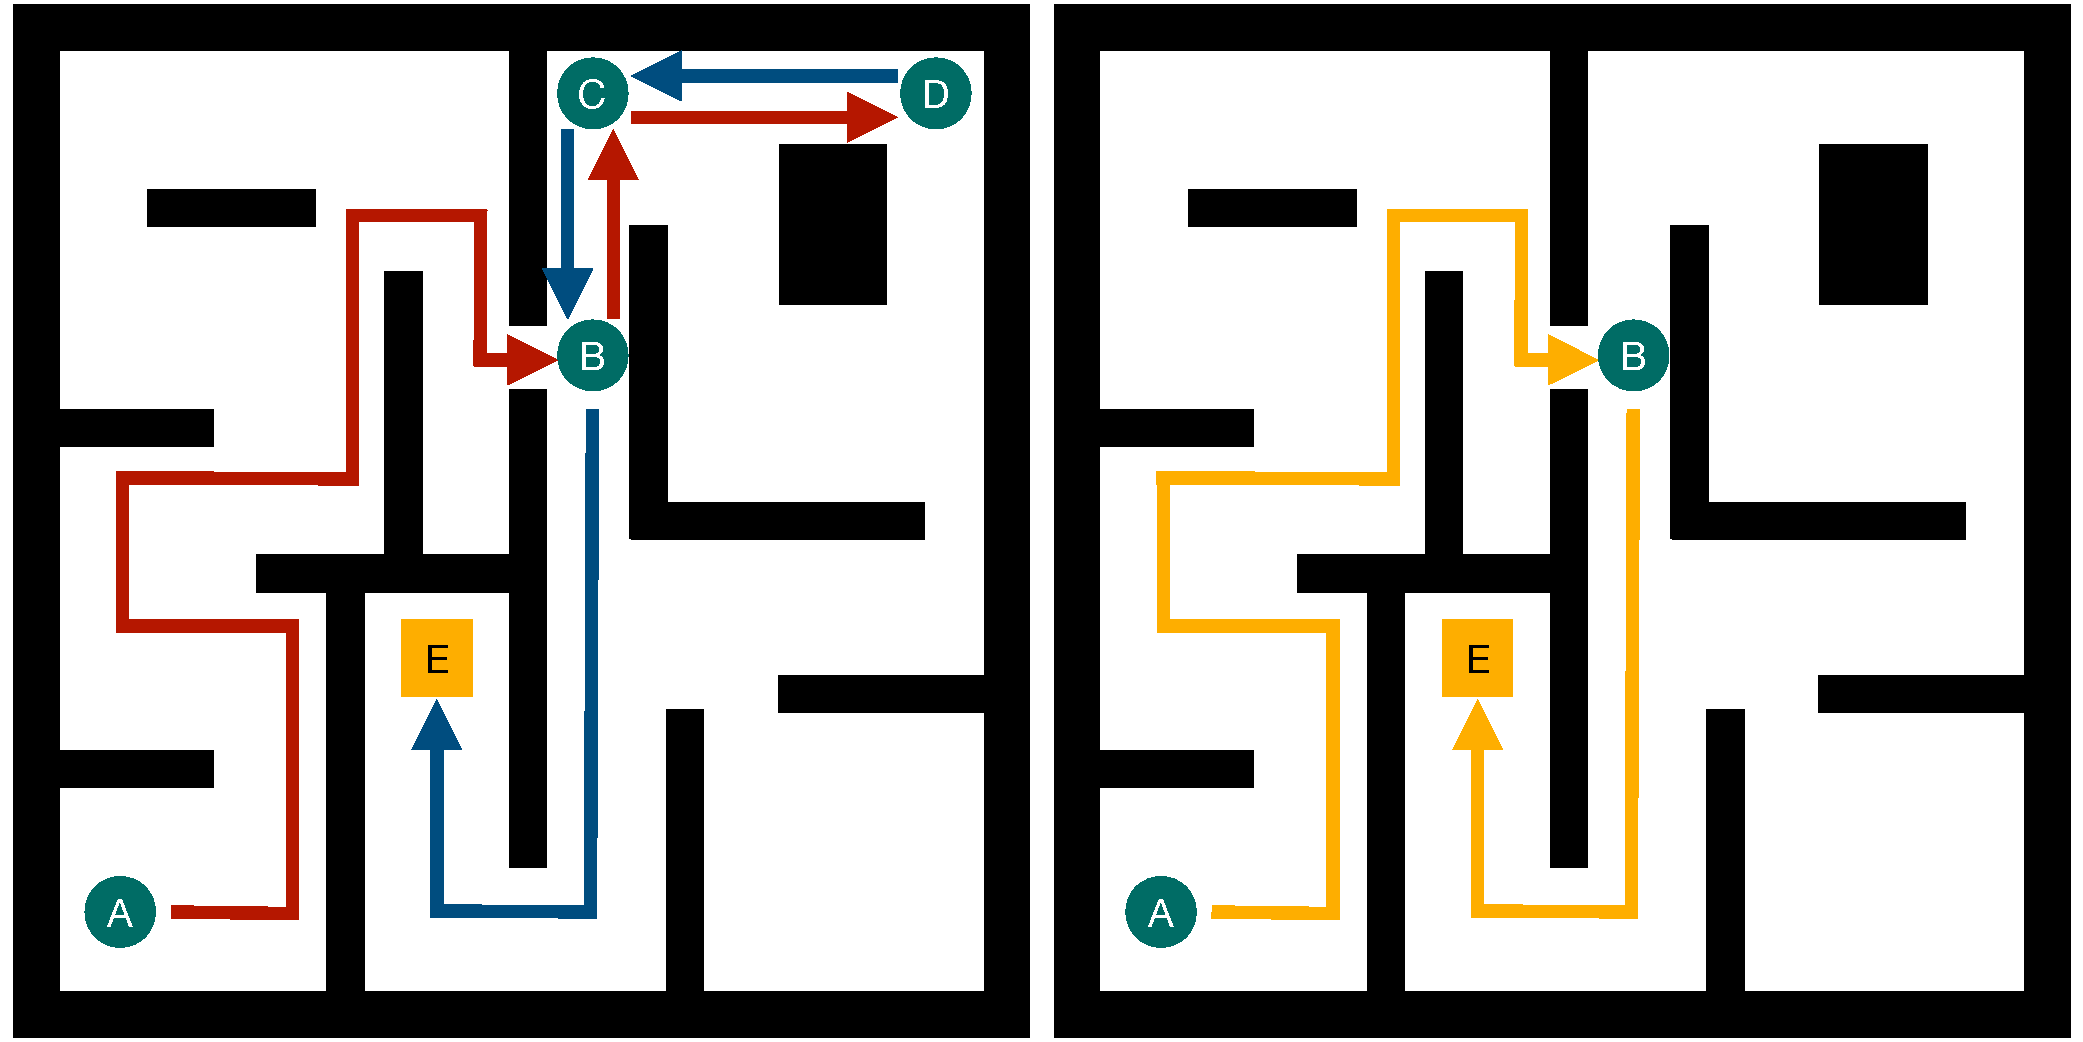
\includegraphics[width=0.6\linewidth]{images/maze_stitching.pdf}
    \caption{Visualization of the stitching process in Offline Reinforcement Learning. In the dataset, 
    we originally observe only partial trajectories—specifically, the segments from $ A \rightarrow D $
    and $ D \rightarrow E $ (as shown on the left). The stitching procedure combines these separate 
    trajectories to construct a new, potentially optimal path from $ A $ to the goal $ E $, 
    even though this complete path was never explicitly observed in the data. Inspired from 
    \cite{OfflineRL_Or_Imitation}}
    \label{offline_stitching}
\end{figure}
At first glance, Offline RL might seem quite similar to Imitation Learning (IL), since both involve learning 
from precollected datasets. This raises the question: can stitching also occur in IL methods?\newline
The key difference between the two settings lies in the availability of reward signals. Offline RL has access
to reward information, which enables the agent to distinguish between good and bad segments of behaviour. This
allows it to selectively stitch together high-quality parts of trajectories to construct better policies.\newline
In contrast, Imitation Learning typically does not have access to rewards. It relies solely on mimicking the observed 
behaviour, making it difficult to identify which parts of a trajectory are optimal or suboptimal. As a result, IL may end up 
stitching together poor behaviours or failing to prioritize the best ones. 

\subsection{Challenges in Offline-RL}
One problem that Offline-RL suffers from is overestimation. In 
\cite{kumar2019stabilizingoffpolicyqlearningbootstrapping} they did an experiment where 
they collected data from an agent that had been trained with some sort of SAC and had 
achieved reasonably good results. They used the data generated by this agent to fill a 
replay buffer which then was used for doing Offline-RL on the same task. As you can see in 
figure \ref{off_rl_overestimation}, the actual return is really bad while the Q values are 
very high. So the Offline-RL agent is certain that it actions will lead to high reward but 
in reality the opposite is true. In the following, we will explore from where this problem arises
and discuss potential strategies to mitigate it.
\begin{figure}[H]
    \centering
    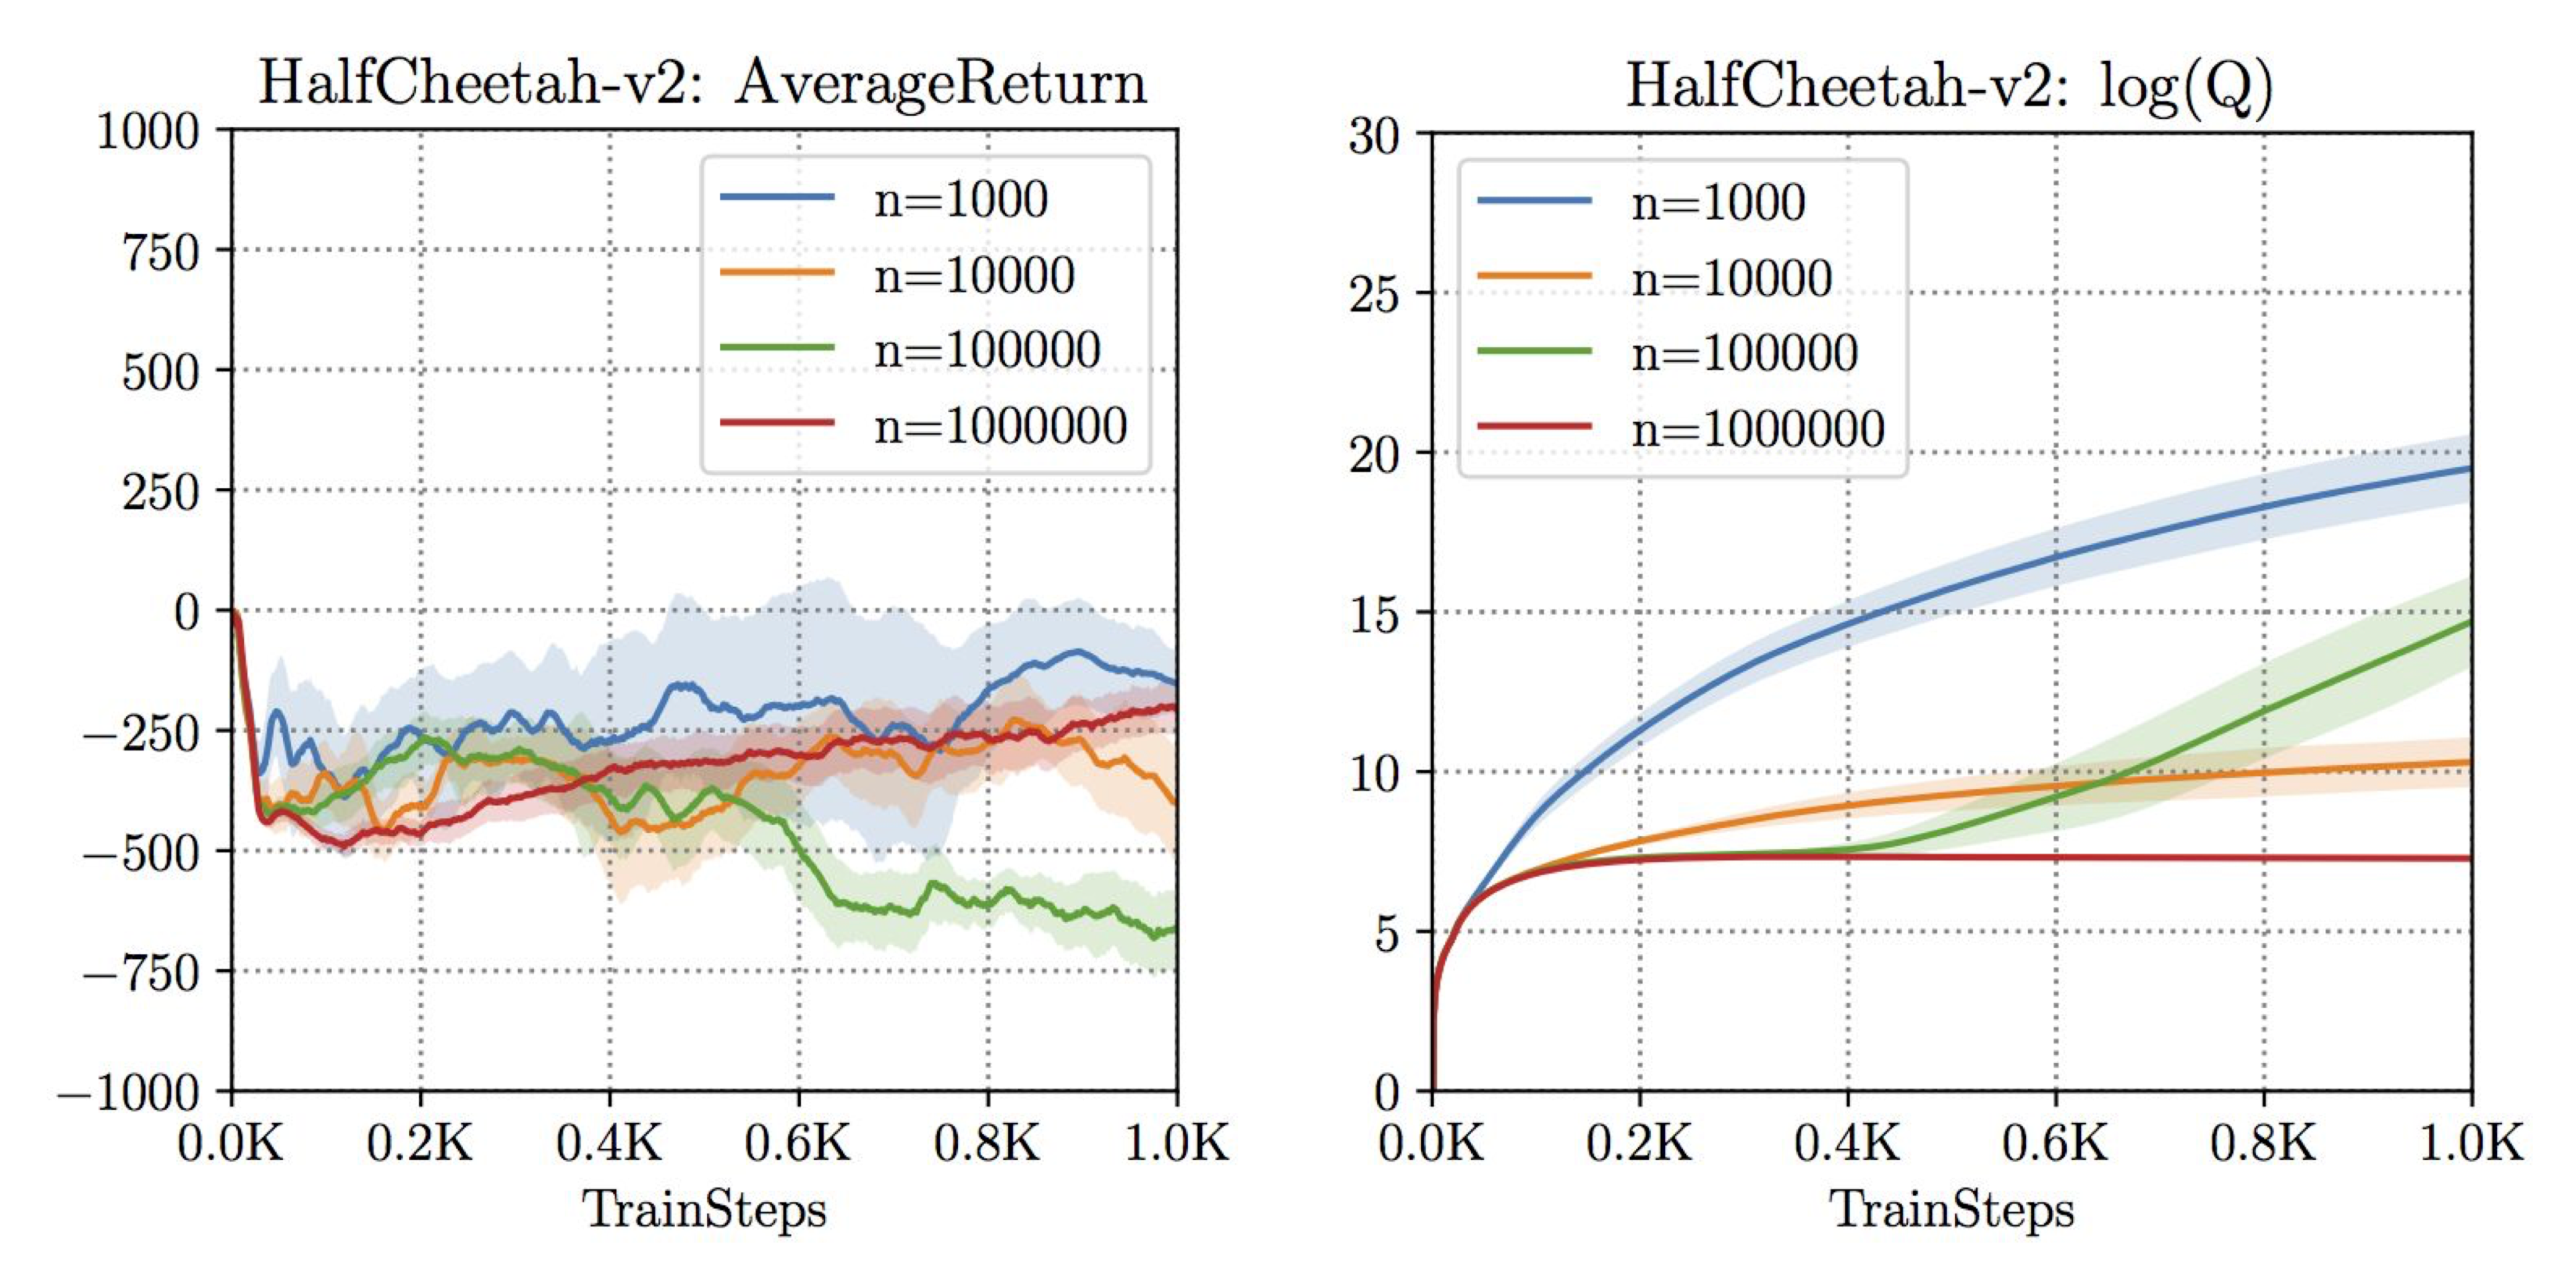
\includegraphics[width=0.72\linewidth]{images/off_rl_problem.png}
    \caption{Performance of SAC on HalfCheetah task with off-policy expert data 
    w.r.t. number of training samples (n), from \cite{kumar2019stabilizingoffpolicyqlearningbootstrapping}}
    \label{off_rl_overestimation}
\end{figure}

\subsubsection{Intuitive Explanation}
The intuitive way to understand the challenge of Offline RL is through counterfactuals. Counterfactuals 
are if statements where the if part is not realised. For example, you are on your way home 
and arrive at a fork in the road where you can either go left or right. Both ways lead to 
your home. So you decide to go left, thinking it would be faster, only to learn that you will
get stuck in traffic and arrive home late. The counterfactual is now ''I should have went right``,
or in other words, ''If I had went right, it would have been better``, even though you do not know
the outcome of going right because you never took it. The core problem is that you are making 
assumptions about the outcomes of actions based solely on the outcomes of the actions you have 
taken without ever observing what would have happened had you chosen differently.\newline 
In Offline RL, such reasoning is necessary. Because for Offline RL to produce policies that outperform
the behaviour seen in the dataset it must consider actions beyond those explicitly observed in the data.
So when updating/executing the policy/Q-values, we typically compare all possible actions in a given state to 
identify the best one. This inherently involves counterfactual reasoning. Because the action we believe 
to be optimal, because it has the highest predicted Q-value, might never been actually observed in the dataset.
If we select it anyway, we are relying entirely on predictions, with no evidence to back them up and so doing
counterfactual reasoning.\newline 
However, counterfactual reasoning in Offline RL brings about a deeper, more subtle problem: distributional shift which 
we already saw when we looked at Imitation Learning and Model-Based-Reinforcement-Learning. Offline RL inherently involves 
making predictions about what would happen under a different policy than the one that generated the data. So it seeks 
to learn a new policy that deviates from the behavior policy ideally to achieve better performance which naturally leads to a 
shift in the distribution of visited states and actions. This shift manifests in two key ways. First, the learned policy may 
visit parts of the state space that were rarely or never seen in the dataset. Second, even in familiar states, it may prefer 
different actions than those taken by the behavior policy (see above explanation). In both cases whether policies, value 
functions, or models—are forced to make predictions under conditions different from those they were 
trained on (distributional shift).\newline
Unlike online RL methods, which can try the action and learn from its outcome, offline methods do not have this luxury. As a 
result, Offline RL must find ways to handle uncertainty around unseen actions (out-of-distribution (OOD)) typically by 
regularizing, constraining, or penalizing those actions during learning.

\subsubsection{Mathematical Explanation}
We now turn to the mathematical explanation of the problem. In general machine learning, our objective is 
typically framed as risk minimization:
 $$\theta \gets \argmin\limits_\theta \mathbb{E}_{x\sim p(x),y \sim p(y|x)}[(f_\theta(x)-y)^2]$$
After training, we might ask: Given a new input $x^*$, is the model's prediction $f_\theta(x^*)$ likely to be accurate?
In expectation, the error is low but only if $x^* \sim p(x)$  so if it comes from the same distribution as the training data. 
If $x^*$ is drawn from a different distribution, this guarantee no longer holds.\newline 
Moreover, if we move away from evaluating under expectation and consider individual inputs, we lose even more certainty. We 
can not guarantee low error, even if $x^*$ was from the training set. This can be easily exploited if we choose 
$x^* \gets \argmax\limits_x f_\theta(x)$.\newline 
In methods like Q-Leaning- or Actor-Critic-methods, we compute the target values $y$ under some policy $\pi_\text{new}$ and try to regress them onto the Q-values
\begin{gather*}
    Q^{k+1}= \argmin\limits_Q \mathbb{E}_{s,a,s' \sim D \sim {\color{cyan}\pi_\beta}}[(Q(s,a)-y(s,a,s'))^2] \\
    \text{with }y(s,a,s') = r(s,a)+\mathbb{E}_{a' \sim {\color{red}\pi^k}}[Q^k(s',a')] \qquad (\text{see footnote \footnotemark})
\end{gather*}
Similar to above, we expect the Q values to be accurate if $\pi^k(a|s) = \pi_\beta(a|s)$. But the whole point of offline-RL is that $\pi^k \gg \pi_\beta$, and to make matters worse, in most methods we choose 
 $$\pi^{k+1} = \argmax\limits_\pi \mathbb{E}_{s\sim D,a\sim \pi^k(a|s)}[Q^{k+1}(s,a)]$$ so we are explicitly trying to find actions that produce high Q values.
 \footnotetext{
$y = r(s,a)+\mathbb{E}_{a' \sim {\pi^k}}[Q^k(s',a')]$ may seem unfamiliar at first, as we initially defined the targets as 
$r(s,a) + \gamma \max\limits_{a'} Q^k(s', a').$
However, we can rewrite this expression as
$r(s,a) + \gamma Q^k\left(s', \arg\max_{a'} Q^k(s', a')\right),$
which, using the relationship in Equation~\eqref{eq:v_to_q}, leads us back to the same formulation.
 }


 \subsection{Approaches to Offline-RL}
%There are several ways to deal with this overestimation problem in offline-RL. The oldest, 
%but no longer used, methods are to use important sampling or linear fitted value 
%functions, while current methods use policy constraints, which we will look at 
%next.\newline
The most common approach for addressing the distributional shift problem in Offline-RL is to impose constraints on how much 
the learned policy is allowed to deviate from the behaviour policy, leading to an optimization objective of the form:
$$\pi_\text{new} = \argmax\limits_\pi \mathbb{E}_{a\sim \pi(a|s)}[Q(s,a)] \quad 
\text{s.t.} \quad \text{Diff}(\pi||\pi_\beta)\leq \epsilon$$ 
This approach comes with two key challenges. First, the constraint may not be pessimistic enough. Even if two policies are 
close in terms of a divergence metric (like KL), they can still differ significantly at specific states. This means the 
learned policy might take actions in certain states where the Q-values are poorly estimated, leading to unreliable 
behaviour.\newline 
Second, if the constraint is too pessimistic, it can prevent the learned policy from meaningfully improving over the behaviour 
policy. In such cases, the policy is forced to stay so close to $\pi_\beta$ that it cannot explore better actions, limiting 
its potential to exceed the performance of the dataset policy.\newline 
For simplicity, in the following we always use the KL as the distance measure for the 
constraint, but it also can be any other measure for probabilities.\newline
To better understand the second challenge, consider Figure \ref{out_of_support}.  We are given the behaviour policy $\pi_\beta$ (blue) for a single 
state. The blue dots represent samples from our data set where y values correspond to q values. The q-function fitted to 
these samples is given by the orange function. If we now train a policy that maximises the q values but also satisfies the 
constraint, we get $\pi_\text{KL}$ (red). You can see that this policy does not only focus on the actions with the highest 
q-values, but also assigns non-negligible probabilities to actions with low q-values. The reason for this is that the KL 
constraint forces it to be something like $\pi_\beta$. Intuitively, we would want something like $\pi_\text{support}$ (green),
but that violates the constraint because the variance is so far off.\newline 
What comes closer to what we want but is more difficult to implement are support constraints 
$$\pi(a|s) > 0 \iff \pi_\beta(a|s) \geq \epsilon $$
\begin{figure}[H]
    \centering
    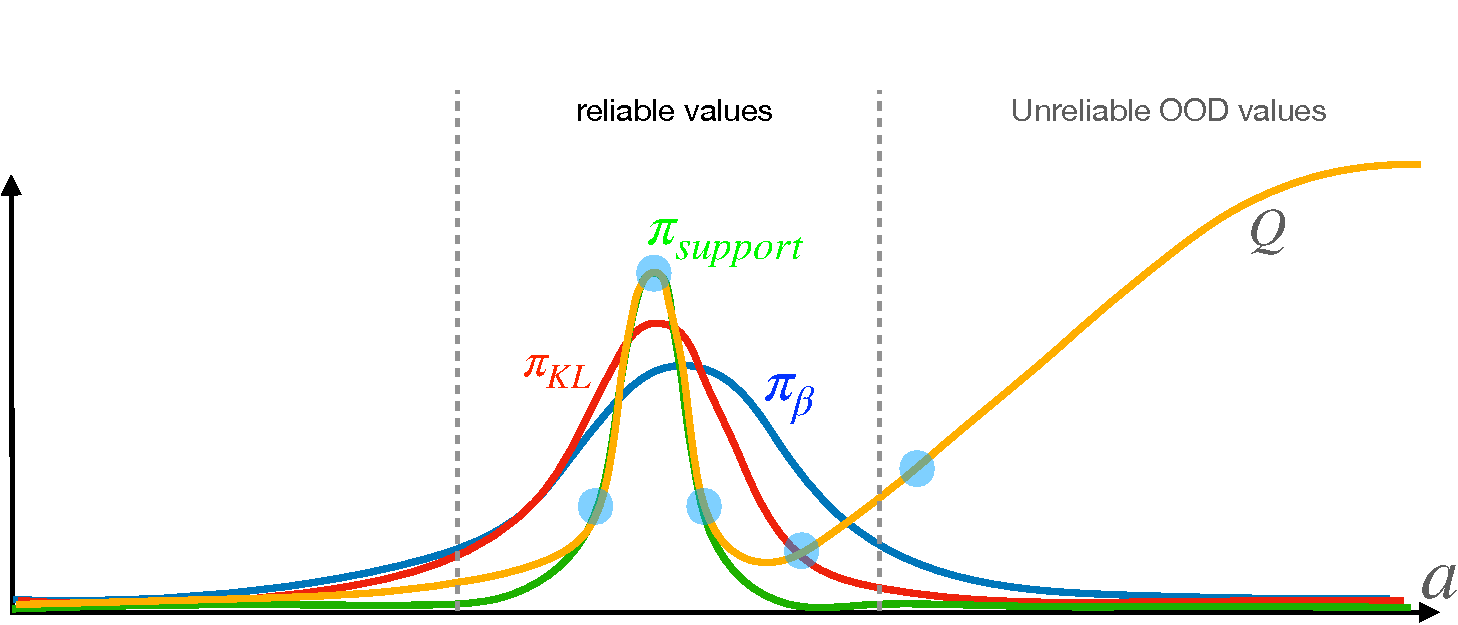
\includegraphics[width=0.8\linewidth]{images/explicit_offline_rl.pdf}
    \caption{Visualization of explicit policy constraints using KL divergence. Inspired by CS 285: Lecture 16 \cite{CS285,CS285LevineYoutube}.}
    \label{out_of_support}
\end{figure}
\subsubsection{Explicit Policy Constraints}
One common approach to incorporating policy constraints in Offline RL is to solve the constrained optimization problem using 
the method of Lagrange multipliers. This leads to the following objective:
\begin{align*}
     \pi_\text{new}(a|s) &= \argmax\limits_\pi \mathbb{E}_{a\sim \pi(a|s)}[Q(s,a)] - \lambda \text{KL}(\pi||\pi_\beta) \\
     %&= \argmax\limits_\pi \mathbb{E}_{a\sim \pi(a|s)}[Q(s,a)] - \lambda \mathbb{E}_{\pi}[\log{\pi(a|s)}-\log{\pi_\beta(a|s)}] \\
     %&= \argmax\limits_\pi \mathbb{E}_{a\sim \pi(a|s)}[Q(s,a)] - \lambda \left(-H(\pi(a|s))-\mathbb{E}_\pi(\log{\pi_\beta(a|s)})\right) \\
      &= \argmax\limits_\pi \mathbb{E}_{a\sim \pi(a|s)}[Q(s,a)+\lambda \log{\pi_\beta(a|s)}] + \lambda H(\pi(a|s)) 
\end{align*}
Here, the Lagrangian multiplier $\lambda$ can either be computed via dual optimization or treated as a hyperparameter. 
However, since we're not solving for the policy in closed form, we simply optimize the objective directly. An alternative idea 
is to incorporate the constraint directly into the reward function:
$$r_\text{diff}(s,a) =r(s,a)- \text{KL}(\pi||\pi_\beta)$$
While this explicit approaches using KL constraints are simple to implement, they rely on access to the behaviour policy $\pi_\beta$ which is often unknown in practice. One idea is to learn $\pi_\beta(a|s)$ from the data via a model. Another idea is to cleverly implement the constraint that we only need access to the samples, not the probabilities which we will looking at in the following.

\subsubsection{Implicit Policy Constraints}
When we once again express the constrained objective using the Lagrangian and this time solve for the optimal 
policy in closed form, we obtain:
$$\pi^*(a|s) = \frac{1}{Z(s)}\pi_\beta(a|s)\exp{\frac{A^{\pi_\text{old}}(s,a)}{\lambda}}$$ 
Here $Z(s)$ is the normalizing constant to ensure the result is a valid probability distribution, and $\lambda$ is the 
Lagrangian multiplier. This optimal policy can now be approximated via maximum likelihood estimation, yielding the 
following objective:
$$\pi_\text{new}(a|s)= \argmax\limits_\pi \mathbb{E}_{(s,a)\sim \pi_\beta}\left[\frac{1}{Z(s)}\log{(\pi(a|s))}\exp{\frac{A^{\pi_\text{old}}(s,a)}{\lambda}}\right]$$
Notably, this formulation does not require explicit evaluation of $\pi_\beta$ only to draw samples from it.
However, it still suffers from the problem of out-of-distribution actions, as computing advantages using Q-values requires 
querying actions that lie outside the behaviour policy’s distribution. In the following 
we will look at methods which try to completely avoid outer distribution action in the Q-update and so
preventing the overestimation issue.

\subsubsection{Implicit Q-Learning}
The update rule for the Q-function can be expressed using the value function as follows:
$$Q(s,a) \gets r(s,a)+\gamma \mathbb{E}_{a'\sim \pi_\text{new}}
[Q(s',a')]\overset{eq. \eqref{eq:v_to_q}}{=} r(s,a)+\gamma V^{\pi_\text{new}}(s')$$ 
We assume that $V(s') $ is represented by a neural network. When we regress $ V $ onto $ Q(s, a) $ 
using mean squared error (MSE) as we've done previously we end up approximating the Q-function 
corresponding to $ \pi_\beta $, since our dataset is generated by $ \pi_\beta $. Thus, we are effectively learning 
$ Q_{\pi_\beta} $ rather than $ Q_{\pi_\text{new}} $.\newline
An important observation is that, in large or continuous datasets, individual states are often visited only once, with 
typically a single action taken per state. However, nearby similar states may be visited with different actions. In practice, 
the policy generalizes across such states, meaning the targets are not fixed values but rather form a distribution (see 
Figure~\ref{v_value_dist}).
\begin{figure}[H]
    \centering
    \resizebox{!}{5cm}{
\begin{tikzpicture}[
    declare function={binom(\k,\n,\p)=\n!/(\k!*(\n-\k)!)*\p^\k*(1-\p)^(\n-\k);}
]
\begin{axis}[ymin=0, xmin=-0.5,axis lines=left,xlabel={$V(s)$}, xticklabels={},yticklabels={,,} ,ylabel={$P(V(s))$}, x label style={at={(axis description cs:1,0.1)},anchor=north},
    y label style={at={(axis description cs:-0.15,1)},rotate = -90, anchor=north}, ,
    samples at={0,...,12},
    yticklabel style={
        /pgf/number format/fixed,
        /pgf/number format/fixed zerofill,
        /pgf/number format/precision=2
    },
    ybar=0pt, bar width=1, bar shift=0pt
]
\addplot [fill=gray!25,] {binom(x,12,0.4)}; 
\addplot [fill=gray!25, samples at={0,...,4}] {binom(x,12,0.4)};
\addplot [fill=gray!25, samples at={7}] {binom(x,12,0.4)};
\def\ymin{\pgfkeysvalueof{/pgfplots/ymin}}
  \def\ymax{\pgfkeysvalueof{/pgfplots/ymax}}
  \draw[ultra thick, dashed,color = cyan] 
    ($(axis cs:7, \ymin)!.5!(axis cs:9, \ymin)$) -- 
    ($(axis cs:7, 0.25*\ymax)!.5!(axis cs:9, 0.25*\ymax)$)
  ;
    \draw[ultra thick, dashed,color = red]
    ($(axis cs:4, \ymin)!.9!(axis cs:5, \ymin)$) --
    ($(axis cs:4, 1.2*\ymax)!.9!(axis cs:5, 1.2*\ymax)$) node[] {Your Text Here}
  ;

\end{axis}
\end{tikzpicture}}
\caption{Probability distribution of the value function for a given state}
\label{v_value_dist}
\end{figure}
When performing MSE regression, the model tends to predict the mean of the value distribution represented 
by the red dashed line. However, what we actually want is to focus on the upper quantile, where the value
under the optimal policy is supported by the data (illustrated by the cyan dashed line).  
To achieve this Implicit-Q-Learning \cite{kostrikov2021offlinereinforcementlearningimplicit} uses the expectile 
regression loss, defined as:
$$L_\text{expectile}(x) = 
\begin{cases}
(1-\mu)x^2,\quad \text{if } x> 0\\ \mu x^2\qquad\qquad \text{else} 
\end{cases}$$ 
The purpose of this loss function is to penalize negative errors more heavily than 
positive ones, encouraging predictions of higher values. At first glance, this may appear 
to contradict the goal of avoiding overestimation. However, overestimation does not occur 
in this case because all the actions we take are drawn from within our dataset, ensuring 
that no out-of-distribution (OOD) actions are involved. As a result, we can update our Q-
functions without the risk of out-of-distribution actions.\newline
What can be shown is that this implicit Q-learning corresponds to support constraints:
$$V(s) \gets \max_{a \in \Omega(s)} Q(s,a) \quad \text{with} \quad \Omega(s) = \{a:\pi_\beta(a|s)\geq \epsilon\}$$

\subsubsection{Conservative Q-Learning}
Conservative Q-Learning (CQL) \cite{kumar2020conservativeqlearningofflinereinforcement} aims to mitigate overestimation in 
offline reinforcement learning by explicitly penalizing large 
Q-values, especially for out-of-distribution (OOD) actions. The core idea is to modify the Q-learning objective as follows:
$$Q^\pi = \argmin\limits_Q \mathbb{E}_{(s,a,s')\sim D}\left[\left(Q(s,a)-(r(s,a)+\mathbb{E}_\pi[Q(s',a')])\right)^2\right] + \max_\mu \alpha \mathbb{E}_{s\sim D, a\sim \mu(a|s)}[Q(s,a)] $$ 
Here, the second term penalizes large Q-values under some auxiliary policy $\mu$, encouraging conservatism by lowering Q-
values for actions not present in the dataset $D$.\newline
However, this approach can become overly pessimistic-reducing all Q-values, including those that are not overestimated. To 
address this, a corrective term is introduced that subtracts the expected Q-value over the dataset distribution. The full CQL 
loss becomes:
\begin{align*}
    Q^\pi =\argmin\limits_Q \mathbb{E}_{(s,a,s')\sim D}\left[\left(Q(s,a)-(r(s,a)+\mathbb{E}_\pi[Q(s',a')])\right)^2\right] &+ \underbrace{\max_\mu \alpha \mathbb{E}_{s\sim D, a\sim \mu(a|s)}[Q(s,a)]}_{\text{punish big Q-values}} \\&- \underbrace{\alpha \mathbb{E}_{(s,a)\sim D}[Q(s,a)]}_{\text{unless they from dataset}}
\end{align*}

%Thus, Conservative Q-Learning follows the following loop:
%\begin{enumerate}
%    \item update $Q^\pi$ w.r.t. $L_{CQL}$ using dataset $D$
%    \item update policy $\pi$
%\end{enumerate}

\subsection{Resources}
This section is largely based on Sergey Levine’s CS 285 ''Lecture 15 – Offline Reinforcement Learning`` and ''Lecture 16 – Offline Reinforcement Learning 2``\cite{CS285,CS285LevineYoutube}. For a more in-depth comparison between Offline Reinforcement 
Learning and Imitation Learning, see \cite{kumar2022preferofflinereinforcementlearning}.
